% ----------------------------------------------------
% Implementation
% ----------------------------------------------------

\chapter{PCB Construction, Adjustments and Code}

\section{PCB Design}

The probe, controller and gold electrodes were fabricated on \glspl{pcb}, which were designed using KiCad software and manufactured with \texttt{JLCPCB}.
The KiCad design files are in the Git repository linked in \refappx{appx:gitrepo}. 
The gold electrodes were trivial, only requiring a single layer \gls{pcb} with simple pads and traces.

The probe \gls{pcb} was the most complex.
It was fabricated on a 4-layer \gls{pcb} with dimensions of $50\times 50mm$, shown in \reffig{fig:probe-pcb}.
\texttt{JLCPCB} offered a discount for 4-layer \glspl{pcb} that were smaller than $50\times 50mm$ in size.
While the probe should ideally be as small as possible to fit through the ice core, it was not designed to be smaller than $50\times 50mm$ to allow for a more straightforward debugging process.

%chktex-file 44
\begin{figure}[ht]
    \begin{minipage}{0.5\textwidth}
        \centering
        \includegraphics[width=0.8\textwidth]{Figures/probe_pcb}
        \caption{The probe PCB with the gold electrodes attached and some adjustments made}
        \label{fig:probe-pcb} %chktex 24
    \end{minipage}
    \begin{minipage}{0.5\textwidth}
        \centering
        \begin{longtblr}[
 caption=\reffig{fig:probe-pcb} Key,
 ]
 {
 hlines,
 colspec = {Q[c,m] Q[l,m,7cm]},
 }
 1 & Programmer Port \\
 2 & Test Points \\
 3 & Pressure Sensor in a Protective Housing \\
 4 & $11\times$ Gain Op-Amp \\
 5 & Titanium Electrode Port \\
 6 & Gold Electrodes \\
 7 & Unity Gain Buffer Op-amp \\
 8 & \gls{dac} and Buffer Transistor \\
 9 & \gls{uart} to \gls{rs485} Converter \\
 10 & \gls{rs485} Port \\
 11 & \gls{uart} Port \\
 12 & STM32F4 Microcontroller \\
 13 & \glspl{led} \\
        \end{longtblr}
    \end{minipage}
    \vspace{0.2cm} \\
    \textit{Note 1: The rest of the titanium electrode ports are behind the gold electrode.} \\
    \textit{Note 2: The other \glspl{ic} present are the TS3A4751 switches.}
\end{figure}

The probe was designed with the resistance measuring circuitry, the temperature and pressure sensors, the microcontroller, the \gls{uart} to \gls{rs485} converter and the \gls{rs485} port mentioned in \refch{ch:design}.
The gold and titanium electrode ports, which were placed at the bottom of the probe, were designed to allow them to be soldered perpendicular to it.
The other methods of attachment all presented a fundamental disadvantage: connecting them with wires added extra resistance, and attaching them parallel to the board or perpendicular facing downwards was considered too complex.

Several adjustments were made to facilitate easier debugging
A \gls{uart} port was added next to the \gls{rs485} port to allow for data to be streamed to a computer using a \gls{uart} to \gls{usb} converter.
Both ports also had reverse polarity protection added to prevent unintentional board damage. 
\glspl{led} were added next to the microcontroller, and a programmer port and test points were added at the top of the board to allow for visual feedback and circuit analysis.
With the programmer and communication ports at the top of the board and the electrodes at the bottom, the probe could safely be submerged while transferring its data to a laptop.

The controller \gls{pcb} was fabricated on a 2-layer board, which is shown in \reffig{fig:controller-pcb}, as the components were too large to fit on a $50\times 50mm$ 4-layer board.
\texttt{JLCPCB} offered a similar discount for 2-layer \glspl{pcb} that were less than $100\times 100mm$ in area.
Ultimately, the controller dimensions were $100\times 60mm$, which could comfortably fit all the components while taking advantage of \texttt{JLCPCB}'s discount.

\begin{figure}[ht]
    \begin{minipage}{0.5\textwidth}
        \centering
        \includegraphics[width=\textwidth]{Figures/controller_pcb_final}
        \caption{The controller PCB with the rotary switch caps attached}
        \label{fig:controller-pcb} %chktex 24
    \end{minipage}
    \begin{minipage}{0.5\textwidth}
        \centering
        \begin{longtblr}[
 caption=\reffig{fig:controller-pcb} Key,
 ]
 {
 hlines,
 colspec = {Q[c,m] Q[l,m]},
 }
 1 & Salinity 7-Segment Display \\
 2 & Depth 7-Segment Display \\
 3 & Rotary Switches \\
 4 & Power Input \\
 5 & \gls{uart} to \gls{rs485} Converter \\
 6 & \gls{rs485} Port \\
 7 & \gls{uart} Port \\
 8 & Input Buttons \\
 9 & Programmer Port \\
 10 & SD Card Port \\
 11 & STM32F0 Microcontroller \\
 12 & \glspl{led} \\
        \end{longtblr}
    \end{minipage}
\end{figure}

The controller was designed with the buttons, the rotary switches, the 7-segment displays, the \gls{uart} to \gls{rs485} converter, and the \gls{rs485} port mentioned in \refch{ch:design}.
The 7-segment displays were designated to display the salinity and depth of the water by default using silkscreen text, but they could be changed to display anything using software.
The components were placed user-friendly, allowing for easy use of the buttons and rotary switches.
Similarly to the probe, \glspl{led}, a \gls{uart} port and a programmer port were added to the board to allow for debugging of the board.
It should be noted that an SD Card Port was added for future development and testing but was not utilised during this project.

\section{PCB Adjustments}

Three adjustments were made to the probe \gls{pcb} to ensure it functioned as required, excluding the soldering of headers and the gold electrodes.
Firstly, one of the microcontroller's pins was unconnected to power and was corrected by soldering a wire between it and a pin with power, which can be seen on the left of the microcontroller.
Secondly, the footprint of the pressure sensor was horizontally reversed, which was corrected by flipping and soldering the depth sensor vertically.
A protective case was added around the pressure sensor to prevent it from being damaged during testing.
The casing would later function as the support for the waterproof membrane mentioned in \refsec{sec:temp-depth-measurement}.

Lastly, both op-amps were incorrectly chosen as they required a rail-to-rail voltage of $6V$ to operate, higher than the $3.3V$ provided.
Thus, they were replaced with an alternative op-amp model with the same footprint.
The temperature sensor also had an incorrect footprint, but this could not be rectified as it was discovered after the board was fabricated. 
Thus, the temperature sensor was not soldered to the board.
The pressure sensor's onboard temperature sensor was used instead.

The controller \gls{pcb} required no soldering adjustments.
There was a minor error in the pin assignments of the rotary switches, but this was corrected in the software and did not require any hardware changes.
Switch caps were 3D printed and attached to rotary switch shafts to make them easier to turn, making the controller more user-friendly.

\section{Probe Code}

The significant steps in measuring salinity are measuring the water's conductivity, temperature and pressure and then calculating its salinity.
An overview of this process is shown in \reffig{fig:probe-code-flowchart}.

\begin{figure}[ht]
    \centering
    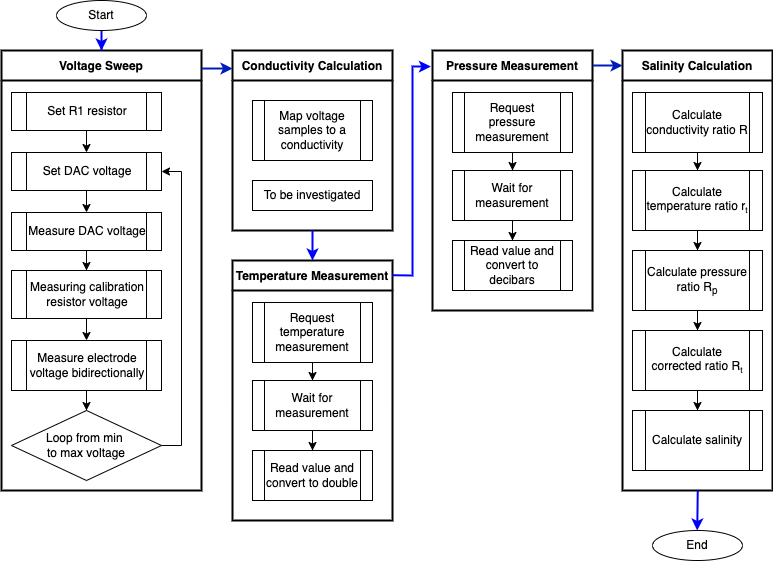
\includegraphics[width=1\textwidth]{Figures/probe_flowchart}
    \caption{The flowchart for the probe code that measures salinity.}
    \label{fig:probe-code-flowchart} %chktex 24
\end{figure}

The conductivity measurement and calculation are different depending on whether the voltage-resistance relationship is constant or not, which is expected for the gold and titanium electrodes, respectively.
Both variations start with a voltage sweep where the \gls{dac} voltage is stepped from the given start voltage to the end voltage.
At each step, the output of the \gls{dac}, the voltage across the calibration resistor and the voltage across the electrodes are recorded.

If the ratio between the \gls{dac} voltage and the voltage across the electrodes is not constant, the conductivity will have to be determined by performing tests to create a model that can relate a set of voltage samples to a conductivity. 
However, if this ratio is constant, the resistance between the electrodes can be calculated using the known calibration $R_1$ resistances as shown in \refeqn{eqn:electrode-calib-resistance} to \refeqn{eqn:electrode-calib-resistance-final}.
The electrode resistances would be calculated for each voltage sample and then averaged, allowing for conductivity to be calculated using \refeqn{eqn:conductivity-from-resistance}.

\begin{align}
 V_{ratio} &= \lfrac{V_{DAC}A_{11}A_{ADC}\lfrac{R_{electrode}}{R_1 + R_{electrode}}}{V_{DAC}A_{11}A_{ADC}\lfrac{R_{calibration}}{R_1 + R_{calibration}}} = \lfrac{\lfrac{R_{electrode}}{R_1 + R_{electrode}}}{\lfrac{R_{calibration}}{R_1 + R_{calibration}}} \label{eqn:electrode-calib-resistance} \\
 \lfrac{R_{electrode}}{R_1 + R_{electrode}} &= V_{ratio} \lfrac{R_{calibration}}{R_1 + R_{calibration}} = k \label{eqn:electrode-calib-resistance-simplified} \\
 R_{electrode} &= \lfrac{kR_1}{1 - k} \label{eqn:electrode-calib-resistance-final}
\end{align}

This method of calculating resistance using a voltage ratio with a known resistance allows the probe to nullify all scalar inaccuracies in the circuit, including the \gls{dac}, \gls{adc} and op-amp gain error, as they will be present in both voltage measurements.
However, this method is still vulnerable to offset inaccuracies, including \gls{dac} and \gls{adc} offset errors, op-amp input offset and input bias currents, the $R_1$ resistance errors and the resistance added by the switches and traces.

As previously mentioned, the pressure and temperature measurements are taken from the WF183DE pressure sensor.
This sensor operates similarly for both measurements: a request is made to make a measure, it can then be polled until the measurement is ready, and then the measurement can be read.

Once the conductivity, temperature and pressure measurements are taken and converted into the required units of $Sm^{-1}$, $\degree C$ and $dbar$ respectively, salinity can be calculated as shown in \refsec{sec:salinity-conductivity-relationship}.
Additionally, if requested, any of the temperature, depth, resistance, or conductivity measurements can be calculated individually and transmitted to the controller.

\section{Controller Code}

The controller's primary function for the prospective user was to instruct the probe to take a measurement and display it. However, the controller was given additional functionality for testing and investigation purposes, which allowed the controller to update the probe's configuration.

The common-cathode 7-segment displays displayed the various measurements from the probe.
The displays' digits were individually written to by writing the digit code and keeping the corresponding digit's cathode low while keeping the others high.
A timer controlled \gls{dma} was used to write to each digit in quick succession, giving the illusion of all the digits being on simultaneously.

The leftmost rotary switch was used to navigate the menu, which consisted of the default showing both salinity and depth, individual measurements of temperature, depth, resistance, conductivity, and salinity, and the probe's configurable parameters.
The menu names were displayed on the top 7-segment display, and the selected menu item was displayed on the other.
This created some limitations on what could be displayed. 
For instance, the best display of the word `temperature' was `teP', but all menu items had a unique, relatively clear name.

When the user selected a measurement menu item, the top switch was configured to request that measurement from the probe and display it; when the user selected a configuration menu item, the top switch was configured to update the probe's configuration.
The other two rotary switches adjusted the probe's configurable parameters, further discussed in \refsec{sec:board-to-board-communication}.
The bottom switch was configured to reset the probe and the controller should an error occur.

\section{Board-to-Board Communication}\label{sec:board-to-board-communication}

The probe and controller communicate using half-duplex \gls{rs485}, which is converted on both sides to \gls{uart}.
This makes the protocol effectively half-duplex \gls{uart} communication from the perspective of the microcontrollers.
The probe was configured to be in receive mode, where it would perpetually wait for a one-byte command from the controller.
All the possible commands and expected transactions are shown in \reffig{fig:rs485-flowchart}.

\begin{figure}[ht]
    \centering
    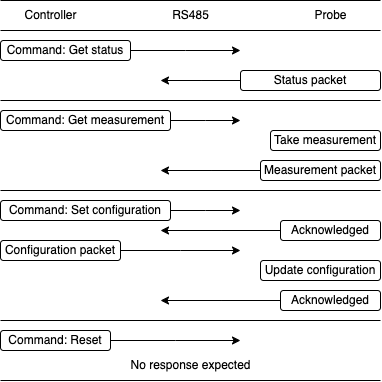
\includegraphics[width=0.5\textwidth]{Figures/rs485_flowchart}
    \caption{The flowchart for the controller code that communicates with the probe.}
    \label{fig:rs485-flowchart} %chktex 24
\end{figure}

While not directly available to the user, the controller could request a status byte to which the probe would respond with \textit{idle}, \textit{busy} or \textit{error} depending on its state.
This allowed for some simple error checking and communication flow, which could be integrated into more robust error handling in the future.
When the user requests a measurement, the controller sends the corresponding request command, to which the probe will respond with the measurement data.
The data was returned as a 3-byte, fixed-point float.

When the user requested a configuration update, the controller transferred a configuration packet using the expected transaction.
Once the probe was entirely cast in epoxy resin, the configuration could only be updated this way, so all possibly useful, configurable parameters are included.
This included which electrode to use (including whether to use the fringe shield), the $R_1$ resistor to use, the directionality of the resistance measurement (unidirectional or bidirectional), the voltage sweep start, end and number of steps, among other parameters.
Some parameters, such as the directionality, were unlikely to be changed from their default value (bidirectional) but were included to cover any unforeseen circumstances.

When the user resets the boards using the controller's bottom switch, a reset command was sent to the probe before the controller reset itself.
This command allows for resetting the probe should a system error occur.
However, this only works provided the \gls{rs485} link is still operational.
Otherwise, the entire system must be powered off and on again to reset the probe.
The reset on both microcontrollers is triggered using software to set the \gls{sys_reset_req} bit in the \gls{scb} register, which triggers a system reset similar to pulling the reset pin low.
